
\documentclass{article}
\usepackage{utf8math,ttquot,mathpartir,amsmath, amssymb, hydrocomments, mathtools,multicol,xspace}
\usepackage[margin=1in]{geometry}
\begin{document}

\abstract{Adding properties to hydroflow is important, because it
  allows us to do three things: (1) it lets us explicitly state and
  verify the requirements individual hydroflow operators have assumed
  of their inputs in order to be correct, (2) It allows us to encode
  translational goals and optimization correctness conditions, and (3) }

\section{technical todo}

\begin{itemize}
\item Type system: basic structure and derivations ✓
\item Type system: properties and their satisfaction
\item semantics: core semantic model (is it rewrite-based?)
\item Type system: axiom rewrite system
\item core language: axiom extensibility
\item proof: progress+preservation (or its equivalent in axiomatic semantics)
\item proof: axiom admissibility (via bisimulation?)
\item evaluation: example programs which satisfy the above
\item evaluation: programmability assessment
\item evaluation: extensibility assessment (new operators)
\end{itemize}

\section{syntax}

\newcommand{\closedprogram}{\textit{closed-program}\xspace}
\newcommand{\compiledcomponent}{\textit{compiled-component}\xspace}
\newcommand{\incast}{\textit{incast}\xspace}
\newcommand{\outcast}{\textit{outcast}\xspace}
\newcommand{\seqstart}{\textit{seq-start}\xspace}
\newcommand{\seqend}{\textit{seq-end}\xspace}
\newcommand{\chain}{\textit{chain}\xspace}
\newcommand{\op}{\textit{op}\xspace}
\newcommand{\opt}{τ_{\textit{op}}\xspace}
\newcommand{\N}{ℕ}
\newcommand{\fresh}{\textit{fresh}\xspace}
\newcommand{\inputs}{\textit{inputs}\xspace}
\newcommand{\outputs}{\textit{outputs}\xspace}

\begin{figure}
  \begin{align*}
    \closedprogram &:= "declare"~ A…~"in"~ p\\
    A &∈ \textit{handoff-names}\\
    p &:= [p]\op[p] ∣ A ∣ (p|p)
  \end{align*}
  \label{fig:syntax}
  \caption{Syntax}
\end{figure}


In figure \ref{fig:syntax}

\section{types}

\begin{figure}
  \begin{mathpar}

    {\inferrule{A : in(dₐ : τₐ), A : out(dₐ | τₐ),… ;. : ⊤ ⊢ p : τ}
      {⊢ "declare"~A…~"in"~p : τ}}
    
    {
      \inferrule{\inputs(\op) = τ' \\ \outputs(\op) = τ_o \\
        C;. : ⊤ ⊢ p : τ' \\ C;d.p.\op[0] :^r τ_o ⊢ p' : τ_o'}
                {{C,C'};{d : τ} ⊢ [p]\op[p'] : τ_o'}}
    
    {\inferrule[relevant-parallel]
      {C₁;d[n] : τ ⊢ p₁ : τ₁ \\ C₂;d[n+1] :^r τ ⊢ p₂ : τ₂}
      {C₁,C₂;d[n] :^r τ ⊢ (p₁ ∣ p₂) : (τ₁ ∣ τ₂)}}

    {\inferrule[substructural-fallback]
      {C;d : τ' ⊢ p : τ}
      {C;d : τ' ⊢^r p : τ}}

    {\inferrule[general-parallel]
      {C₁;. : ⊤ ⊢ p₁ : τ₁ \\ C₂;. : ⊤ ⊢ p₂ : τ₂}
      {C₁,C₂; . : ⊤ ⊢ (p₁ ∣ p₂) : (τ₁ ∣ τ₂)}}

    {\inferrule[exchange]
      {A : (dₐ : τₐ),  B : (d_b | τ_b) ; d : τ ⊢ p : τ}
      {B : (d_b | τ_b), A : (dₐ : τₐ) ⊢ p : τ}}
      
    {\inferrule[unfold]{A:d',C;d[A/d] : τ ⊢ p}{A:d',C;d : τ ⊢ p}}

    {\inferrule[fold]{A:d',C;d : τ ⊢ p}{A:d',C;d[A/d] : τ ⊢ p}}

    {\inferrule[varref-out]{}{A:out(d : τ);d : τ ⊢ A : τ}}

    {\inferrule[varref-in]{}{A:in(d : τ);. : \_ ⊢ A : τ}}
      
    \end{mathpar}
    %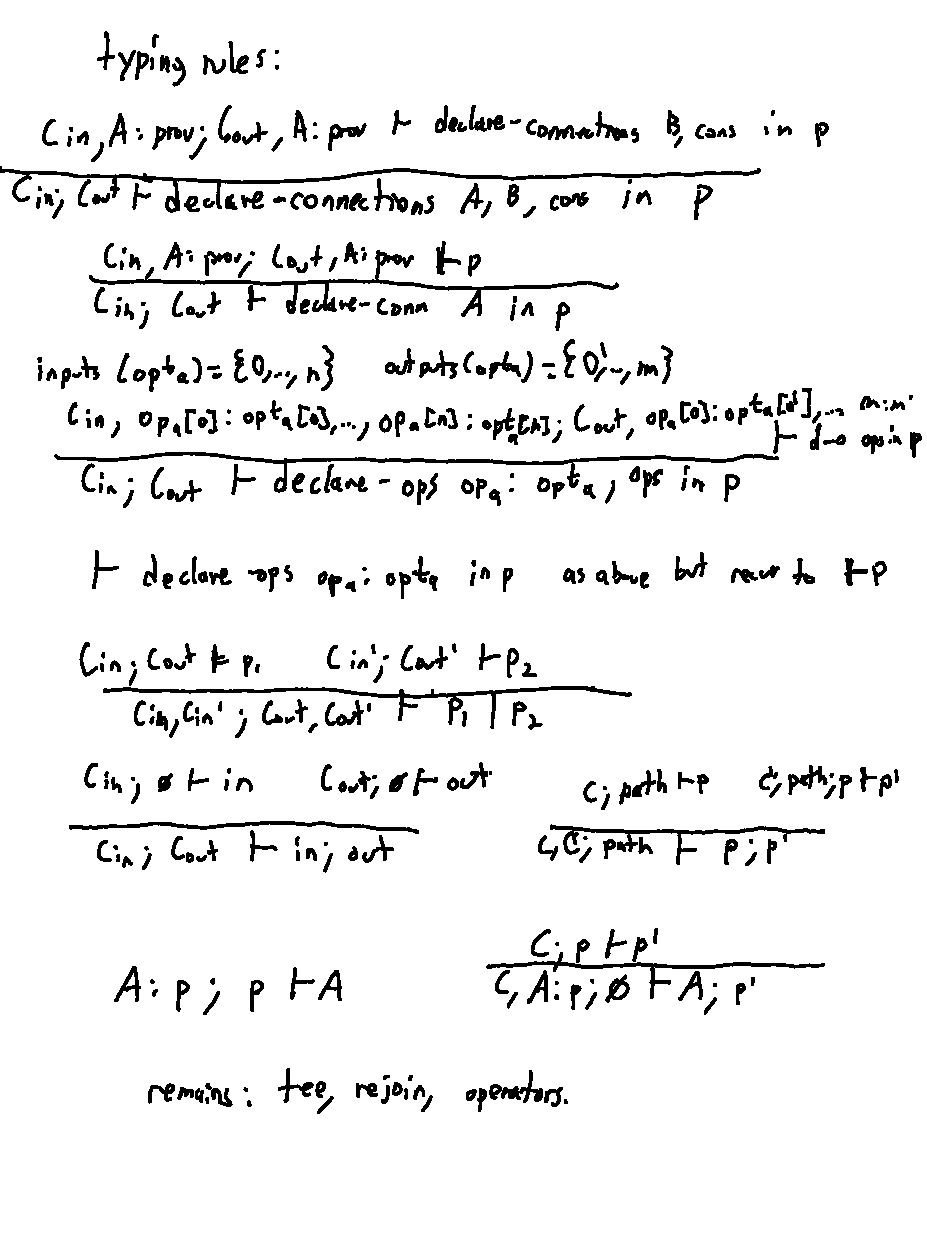
\includegraphics{freehand-types}
  \label{fig:types}
  \caption{Types}
\end{figure}

We're not bothering with the oaklandish split right now, it's too
silly.  Open question if we need the relevance version of the rule, or
can remove the $:^r$ annotation and observe that the $[n]$ version is
only ever used with empty contexts for inputs to operators. Also worth
wondering if we're going to be in trouble overloading the [] syntax
here; time will tell. Types appear in figure \ref{fig:types}


\end{document}
